\documentclass[12pt]{article}
% Эта строка — комментарий, она не будет показана в выходном файле
\usepackage{ucs}
\usepackage[warn]{mathtext}
\usepackage[utf8x]{inputenc} % Включаем поддержку UTF8
\usepackage[russian]{babel}  % Включаем пакет для поддержки русского языка
\usepackage{amsmath}
\usepackage{mathtools}
\usepackage{amssymb}
% \usepackage[dvips]{graphicx}
% \graphicspath{{noiseimages/}}
\usepackage[pdftex]{graphicx}


% Параметры страницы: 1см от правого края и 2см от остальных.


\hoffset=0mm
\voffset=0mm
\textwidth=180mm        % ширина текста
\oddsidemargin=-6.5mm   % левое поле 25.4 - 5.4 = 20 мм
\textheight=240mm       % высота текста 297 (A4) - 40
\topmargin=-15.4mm      % верхнее поле (10мм)
\headheight=5mm      % место для колонтитула
\headsep=5mm          % отступ после колонтитула
\footskip=8mm         % отступ до нижнего колонтитула


\begin{document}
    \author {Жарков Андрей 495}
    \title {Лабораторная работа 2.1 \\  Определение $C_p / C_v$ по скорости звука в газе.}
    \maketitle{}
    
    \begin{center}
    	\textbf{\large{Теория}}
    \end{center}
    \textbf{Цель работы:} 1) измерение частоты колебаний и длины волны
    при резонансе звуковых колебаний в газе, заполняющем трубу;
    2) определение показателя адиабаты по скорости звука с помощью уравнения состояния идеального газа.
    \\ \\
    \textbf{В работе используются:} звуковой генератор (ЗГ); электронный осциллограф (ЭО); микрофон; телефон; раздвижная труба;
    теплоизолированная труба, обогреваемая водой из термостата;
    баллон со сжатым углекислым газом; газгольдер.
    \\ \\
    
    
    \textbf{Звуковые волны.} При распространении звука в газе атомы и
    молекулы колеблются вдоль направления распространения звуковой волны. Это приводит к локальным изменениям плотности
    $\rho$ газа и его давления $P$, поэтому звуковые волны иногда называют волнами плотности или волнами давления.
    В простых гармонических звуковых волнах, распространяю-
    щихся вдоль оси $Ox$, изменение давления $\Delta P$ зависит от коорди-
    наты 𝑥 и времени 𝑡 по закону $$\Delta P(x, t) = P_0 cos(\omega t \pm kx)$$
    Два знака в аргументе косинуса соответствуют двум направлени-
    ям распространения волны. Между круговой частотой $\omega$, волно-
    вым числом 𝑘, длиной волны $\lambda$ и скоростью звука $𝑣_{зв}$ выполняются соотношения 
    \begin{equation}
    v_{зв} = \frac{\omega}{k} = \lambda f ;k=\frac{2\pi}{\lambda}; \omega = 2\pi f
    \end{equation}
    здесь 𝑓 — частота волны.
    
    Важной характеристикой звуковых волн является скорость их
    распространения. Она определяется инерционными и упругими
    свойствами среды. Скорость распространения продольных волн в
    безграничной однородной среде определяется выражением:
    
    \begin{equation}
    v_{зв} = \sqrt{\frac{dP}{d\rho}}
    \end{equation}
    
    Давление 𝑃 зависит не только от плотности $\rho$, но и от температуры 𝑇. Поэтому нужно уточнить, в каком смысле понимается
    производная 𝑑𝑃/𝑑$\rho$.
    Колебания плотности и связанные с ними колебания температуры в звуковой волне происходят настолько быстро, а теплопроводности газов настолько малы, что для таких процессов теплообменом можно пренебречь, так что процесс распространения звука можно считать адиабатическим. Следовательно, производную
    𝑑𝑃/𝑑$\rho$ необходимо рассчитывать для адиабатического процесса.
    
    \textbf{Первое начало термодинамики.} Из закона сохранения энергии следует, что тепло 𝑄, полученное термодинамической системой, расходуется на изменение её внутренней энергии $\Delta U$ и на
    совершение работы 𝐴 над внешними телами:
    \begin{equation}
    Q = \Delta U + A
    \end{equation}
    Данная формула является математической формулировкой первого начала термодинамики. Из неё следует термодинамическое
    определение внутренней энергии и принципиальный способ её измерения: изменение внутренней энергии равно работе, совершённой внешними силами при отсутствии подвода тепла, то есть при
    адиабатическом процессе. Эта энергия состоит из кинетической
    энергии теплового движения молекул и потенциальной энергии
    межмолекулярных и внутримолекулярных взаимодействий.
    
    Для бесконечно малого процесса уравнение (3) принимает вид
    \begin{equation}
    \delta Q = dU + \delta A
    \end{equation}
    
    \textbf{Работа газа.} Рассмотрим расширение газа в цилиндре, закрытом
    подвижным поршнем. На поршень действует сила 𝐹, равная про-
    изведению давления газа 𝑃 на площадь поршня 𝑆. При смещении
    на малую величину 𝑑𝑥 газ совершает работу $\delta$𝐴 = 𝐹𝑑𝑥 = 𝑃𝑆𝑑𝑥 =
    = 𝑃𝑑𝑉 , где 𝑑𝑉 = 𝑆𝑑𝑥 — малое изменение объёма газа.
    
    Таким образом, бесконечно малая работа газа при увеличении
    объёма системы на 𝑑𝑉 равна
    \begin{equation}
    \delta A = PdV
    \end{equation}
    Полная работа в некотором процессе: $$\int P(V)dV$$
    Согласно уравнению состояния давление газа зависит не только
    от его объёма, но и от температуры. Для вычисления работы при
    интегрировании выражения должно быть известно, как изменяет-
    ся температура при изменении объёма, то есть нужно знать весь
    процесс, при котором производится работа, а не только начальное
    и конечное состояния системы.
    
    Первое начало термодинамики для газов после использования
    формулы (5) будет иметь вид
    \begin{equation}
    \delta Q = dU + PdV
    \end{equation}
    \textbf{Теплоёмкость.} Отношение количества тепла $\delta$𝑄, поглощённого
    $\nu$ молями газа при некотором процессе, который обозначим индексом «𝑥», к повышению его температуры на 𝑑𝑇, делённое на
    число молей $\nu$, называется молярной теплоёмкостью газа:
    \begin{equation}
    C = \left(\frac{\delta Q}{dT} \right)_x / \nu
    \end{equation}
    Важно также отметить, что теплоёмкость существенно зависит
    от процесса, при котором происходит подвод тепла, так как часть
    тепла может затрачиваться на совершение работы. Эта работа
    может оказаться столь велика, что теплоёмкость станет отрица-
    тельной, то есть температура тела будет падать, несмотря на то,
    что тепло подводится.
    
    Считая внутреннюю энергию функцией температуры и объёма
    𝑈 = 𝑈(𝑇,𝑉 ), подставим выражение для её дифференциала: $$dU = \left(\frac{\delta U}{\delta T} \right)_VdT + \left(\frac{\delta U}{\delta V} \right)_TdV$$
    в первое начало термодинамики:$$\delta Q = dU + PdV = \left(\frac{\delta U}{\delta T} \right)_VdT + \left(\frac{\delta U}{\delta V} \right)_TdV + PdV = \left(\frac{\delta U}{\delta T} \right)_VdT + \left[P +\left(\frac{\delta U}{\delta V} \right)_T \right] dV$$
    Разделив это соотношение на 𝑑𝑇, найдём теплоёмкость $𝐶_𝑥$ в процессе «𝑥»:
    \begin{equation}
    C_x = C_v + \left[P +\left(\frac{\delta U}{\delta V} \right)_T \right]
    \left(\frac{\delta V}{\delta T} \right)
    \end{equation}
    
    \begin{center}
    	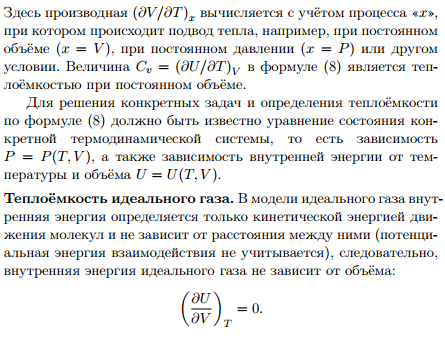
\includegraphics[width=16cm]{theory_0.png}
    	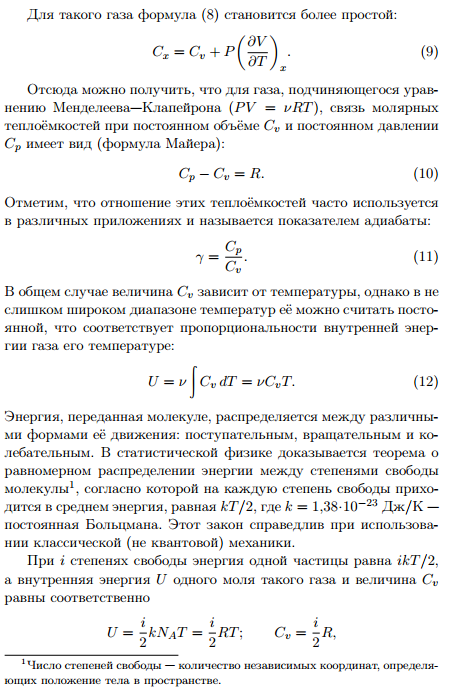
\includegraphics[width=16cm]{theory_1.png}
    	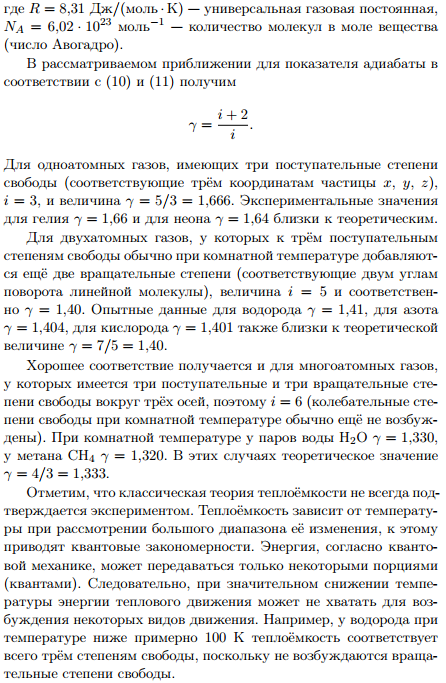
\includegraphics[width=16cm]{theory_2.png}
    	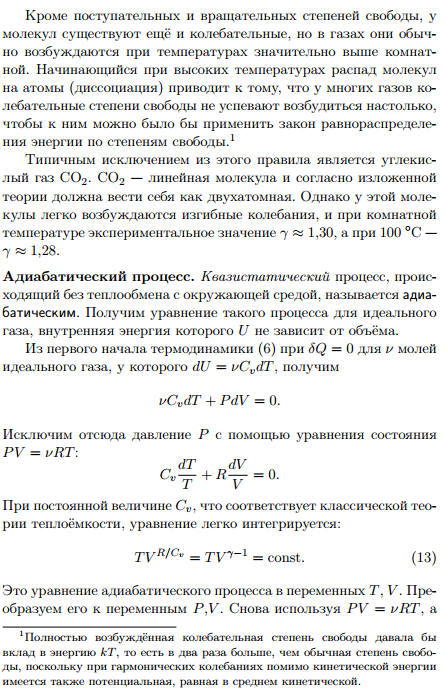
\includegraphics[width=16cm]{theory_3.png}
    	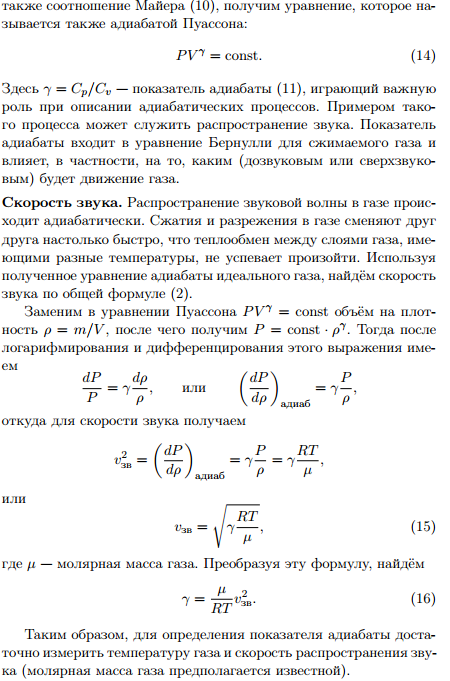
\includegraphics[width=16cm]{theory_5.png}
    	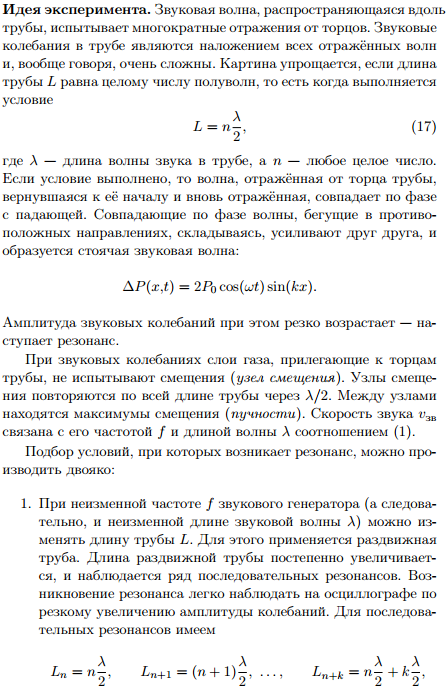
\includegraphics[width=16cm]{theory_6.png}
    	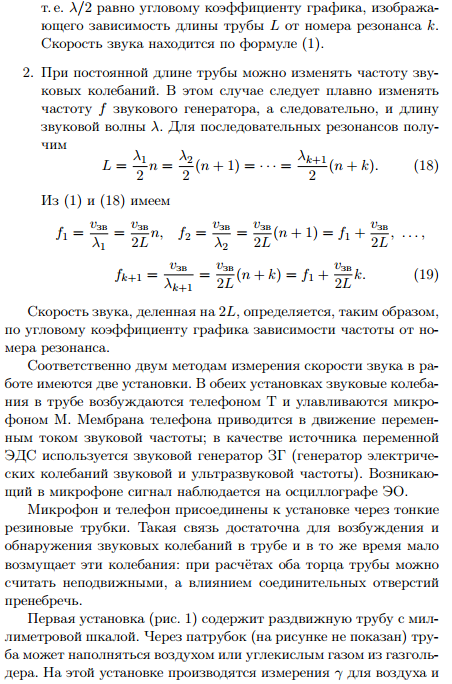
\includegraphics[width=16cm]{theory_7.png}
    	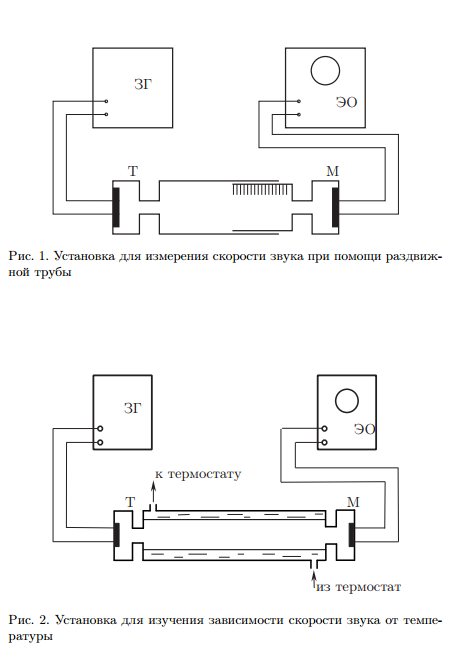
\includegraphics[width=14cm]{theory_8.png}
    	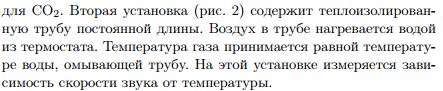
\includegraphics[width=16cm]{theory_9.png}
    \end{center}
    \pagebreak
    \begin{center}
    	\textbf{\large{Выполнение работы}}
    \end{center}
    
    
    \textbf{Измерения при постоянной частоте}
    \\ \\
    Параметры установки: $L_0 = 70,0 \pm 0,5 sm$, $\Delta L_{max} = 23,0 sm$ \\
    Чтобы получить 6 точек на графике рассчитаем частату через $\Delta L_{max} = k\frac{\lambda}{2}$ \\
    Откуда находим рабочую частоту $f \approx \frac{k v_{зв}}{2\Delta L_{max}} \approx 3700 Гц$\\
    Установленная рабочая частота $f = 3698 Гц$\\
    Далее из выдвигаем наполную нашу трубу и медленно сдвигаем, ловя резонансы. Вот что получилось:\\
    
    \begin{center}
    	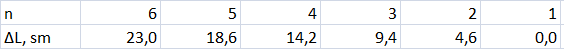
\includegraphics[width=14cm]{table0.png}
    	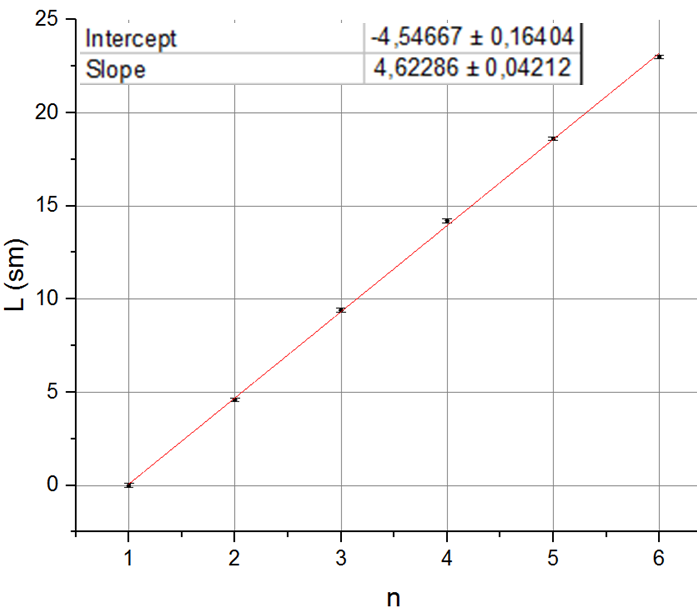
\includegraphics[width=14cm]{graph0.png}
    \end{center}
    Найденный коэффициент наклона графика $k= \frac{\lambda}{2}= (4,62 \pm 0,04) * 10^{-2}$\\
    Теперь можно найти $v_{зв} = \lambda f = 2kf = 342 \pm 3 м/с$\\
    Что в пределах погрешности совпадает с теоретическим значением (при 293 К) $v_{зв} = 343,1 м/с$
    
    
    \pagebreak
    \textbf{Измерения при постоянной длинне трубы}
    
    Параметры установки: $L = 80,0 см$ - длина трубы\\
    Оценим первую резонансную частоту: $f_1 = \frac{v_{зв}}{2L} \approx 206 Гц$ Где-то в этом диапазоне и будем её искать, следующие резонансные частоты будем искать примерно кратно первой найденной.\\
    Погрешность измерения каждой отдельной частоты считаем $\sigma_{f_i} = 10 Гц$\\
    При разных значениях температуры измерены следующие данные:\\
    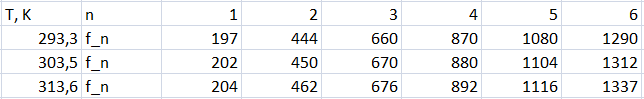
\includegraphics[width=14cm]{table1.png}\\
    \\
    
    \textbf{1. T=293,3K}\\
    \begin{center}
    	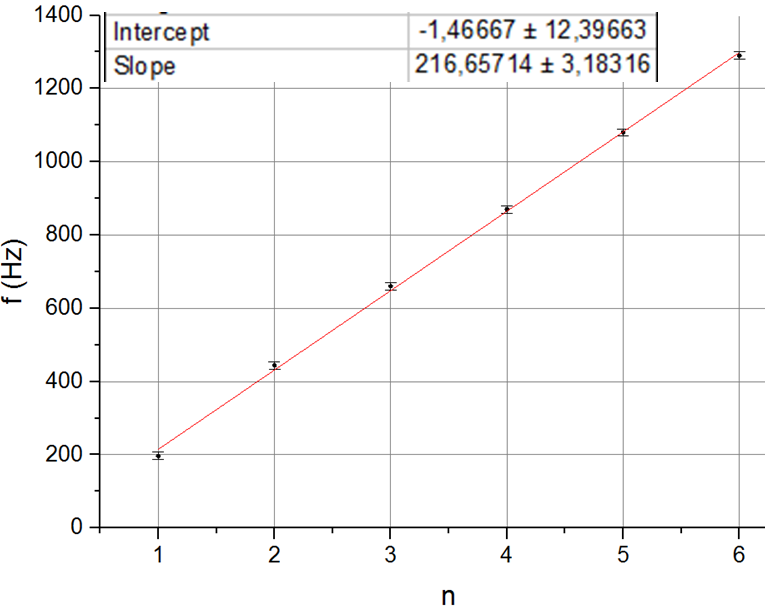
\includegraphics[width=14cm]{graph20.png}\\
    \end{center}
    Найденный коэффициент наклона $k = v_{зв}/2L = 216 \pm 3$
    Находим $v_{зв} = 2kL = 345 \pm 5 м/с$
    Теоретическое значение при данной температуре $v_{теор} = 343,1$\\
    По формуле (16) найдём $\gamma$ ($\mu = 29 г/моль$, $R=8,31$):
    $\gamma = \frac{\mu}{RT}v_{зв}^2 = 1.41 \pm 0.02$, $\gamma_{теор} = \frac{i+2}{i} = 1.4$
    
    \textbf{2. T=303,5K}
    \begin{center}
    	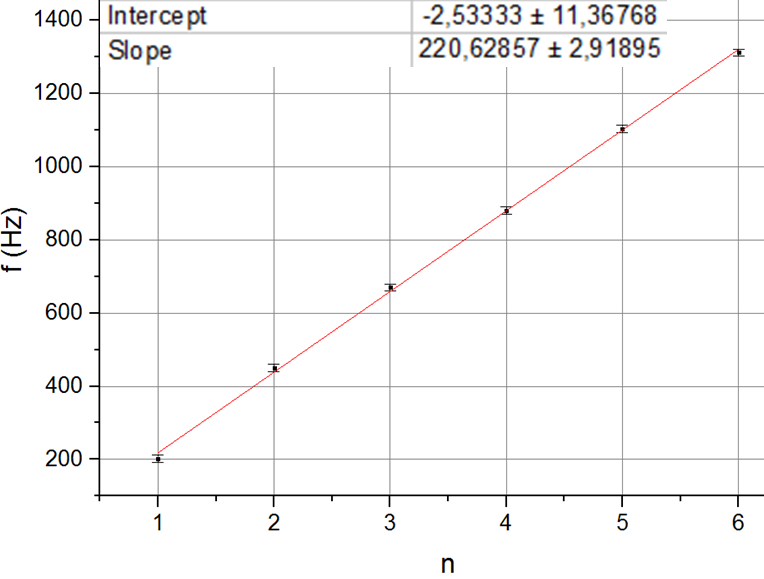
\includegraphics[width=14cm]{graph30.png}\\
    \end{center}
    Найденный коэффициент наклона $k = v_{зв}/2L = 221 \pm 3$
    Находим $v_{зв} = 2kL = 354 \pm 5 м/с$
    Теоретическое значение при данной температуре $v_{теор} = 348,9$\\
    По формуле (16) найдём $\gamma$ ($\mu = 29 г/моль$, $R=8,31$):
    $\gamma = \frac{\mu}{RT}v_{зв}^2 = 1.43 \pm 0.02$, $\gamma_{теор} = \frac{i+2}{i} = 1.4$
    
    \textbf{3. T=316,6K}
    \begin{center}
    	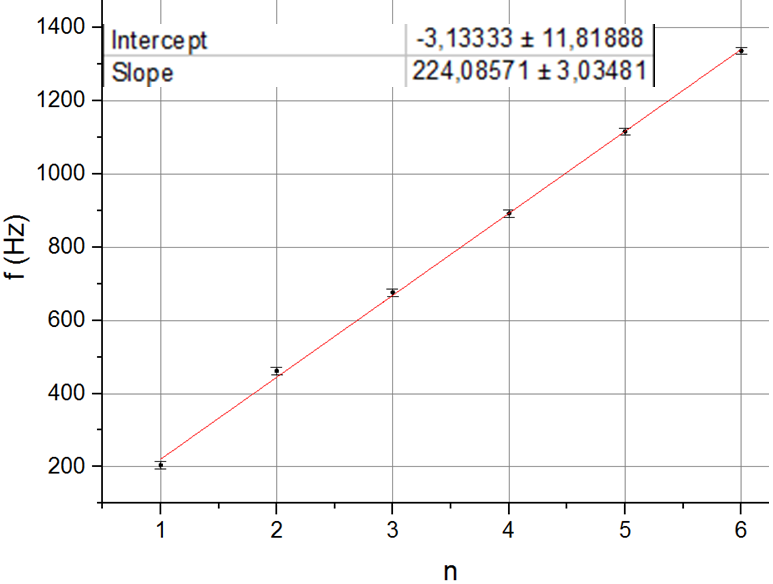
\includegraphics[width=14cm]{graph40.png}
    \end{center}
    Найденный коэффициент наклона $k = v_{зв}/2L = 224 \pm 3$
    Находим $v_{зв} = 2kL = 358 \pm 5 м/с$
    Теоретическое значение при данной температуре $v_{теор} = 354,2$\\
    По формуле (16) найдём $\gamma$ ($\mu = 29 г/моль$, $R=8,31$):
    $\gamma = \frac{\mu}{RT}v_{зв}^2 = 1.41 \pm 0.02$, $\gamma_{теор} = \frac{i+2}{i} = 1.41$
    \\ \\ \\
    Как видим, во всех 3х сериях в пределах погрешности можно принять что найденные значения скоростей звука совпадают с теоретическими.\\
    То же можно сказать и про найденные значения $\gamma$
    
\end{document}